% !TEX root = ../These_Robin_Master.tex
\chapter{Formaliser connaissances et hypothèses, vers un modèle de simulation co-construit : SimFeodal}
\label{chap:chap2}
\begin{center}
	{\large Version \hl{2019-04-12}}
\end{center}

\begin{itemize}
	\item Avril 2019 : Nouveau départ pour le chapitre
\end{itemize}
\setcounter{minitocdepth}{2}
\minitoc

\textbf{Code couleur}
\begin{itemize}
	\item Texte écrit pour cette version du chapitre
	\item {\redroman Texte publié dans le chapitre de Peupler la Terre}
	\item {\blueroman Modifications dans le texte du chapitre de Peupler la Terre}
\end{itemize}

\clearpage

\addcontentsline{toc}{section}{\textit{\textmd{Avant-propos}}}
\begin{mdframed}[backgroundcolor=gray!10,footnoteinside=false]
	\textbf{Avant-propos}\\
Le présent chapitre décrit un modèle, SimFeodal, qui est une œuvre profondément collective et interdisciplinaire.
La paternité de ce modèle est ainsi à attribuer à l'auteur de ces lignes autant qu'à l'ensemble des co-concepteurs du modèle :
\begin{itemize}
	\item Cécile \textsc{Tannier}, UMR 6049 ThéMA -- Besançon\\
	Géographe et modélisatrice, Directrice de Recherche, CNRS
	\item Samuel \textsc{Leturcq}, UMR 7324 CITERES-LAT -- Tours\\
	Historien, Maître de Conférence, Université François Rabelais
	\item Elisabeth \textsc{Zadora-Rio}, UMR 7324 CITERES-LAT -- Tours\\
	Archéologue, Directrice de Recherche émérite, CNRS
	\item Élisabeth \textsc{Lorans}, UMR 7324 CITERES-LAT -- Tours\\
	Archéologue, Professeure, Université François-Rabelais
	\item Xavier \textsc{Rodier}, UMR 7324 CITERES-LAT -- Tours\\
	Archéologue, Ingénieur de Recherche HDR, CNRS

\end{itemize}

Ce chapitre de thèse constitue une reprise, individuelle et largement modifiée et retravaillée, d'un chapitre -- \citetitle{cura_transition_2017} \autocite{cura_transition_2017} -- de l'ouvrage collectif \og Peupler la terre\fg{} \autocite{sanders2018peupler} issu du projet TransMonDyn\footnotemark.
Dans cette thèse, SimFeodal est présenté dans une version différente de celle de l'ouvrage collectif, et de nombreux mécanismes sont par exemple considérablement simplifiés.
Les fondements du modèle, toutefois, restent très largement identiques entre ces deux versions, et à ce titre, ce chapitre de thèse reprend parfois des passages entiers du chapitre de l'ouvrage collectif.
Dans ces moments, nous avons préféré ne pas les identifier en tant que tel, notamment car l'entremêlement de modifications apportées rendrait difficile la lecture.

En matière de forme, notons que contrairement au chapitre publié, le modèle SimFeodal est ici présenté en suivant le protocole de description \og ODD\fg{} (\textit{Overview, Design concepts, and Details}) \autocite{grimm_odd_2010}, dans sa formulation la plus récente (\cite{grimm_documenting_2017}, voir \cref{tab:proto-ODD}).
SimFeodal ne se prête pas à toutes les catégories identifiées par les auteurs de ce standard, et celui-ci n'est de plus pas pensé pour une description aussi détaillée du modèle\footnotemark, mais nous pensons tout de même que le suivi de ce standard d'adoption permettra d'augmenter la reproductibilité de SimFeodal.
Pour cette même raison, notons que l'implémentation du modèle, son historique ainsi que les différentes descriptions techniques sont disponibles dans le dépot de versionnement de SimFeodal :
\begin{center}
	\href{https://github.com/SimFeodal/SimFeodal}{https://github.com/SimFeodal/SimFeodal}
\end{center} 
\end{mdframed}
\footnotetext[1]{
Projet ANR (ANR-10-BLAN-1805), coordonné par Lena \textsc{Sanders}, entre 2011 et 2014.
\href{www.transmondyn.parisgeo.cnrs.fr}{www.transmondyn.parisgeo.cnrs.fr}
}
\footnotetext[2]{
\hl{Une description plus courte, plus proche des descriptions ODD classiques, est disponible en ligne.}
}

\clearpage

\begin{table}[H]
	\centering
	\caption{Les éléments du protocole ODD, d'après \cite[Table 15.1, pp. 353--354]{grimm_documenting_2017}}
	\label{tab:proto-ODD}
	\scriptsize
	{\renewcommand{\arraystretch}{1.5}%
	\begin{tabular}{|p{1.1cm}|p{1.15cm}|p{1.25cm}|p{9.5cm}|}
		\hline
		\textbf{Overview} & \multicolumn{2}{l|}{1. Purpose} & What is the purpose of the model ? \\ \hline
		& \multicolumn{2}{l|}{\pbox[c][24pt][b]{3cm}{2. Entities, state variables, and scales}} & What kind of entities are in the model? Do they represent managers, voters, landowners, firms or something else? By what state variables (attributes or characteristics), are these entities characterized? What are the temporal and spatial resolutions and extents of the model? \\ \cline{2-4} 
		& \multicolumn{2}{l|}{\pbox[c][24pt][b]{3cm}{{3. Process overview and scheduling}}} & What entity does what, in what order?  When are state variables updated? How is time modeled: as discrete steps or as a continuum over which both continuous processes and discrete events can occur? \\ \cline{2-4} 
		\textbf{Design concepts} & 4. Design concepts & Basic principles & Which general concepts, theories or hypotheses are included in the model’s design? How were they taken into account? \\ \cline{3-4} 
		&  & Emergence & What key results are emerging from the adaptive traits, or behaviors of individuals? What results vary in complex/unpredictable ways when particular characteristics change? \\ \cline{3-4} 
		&  & Adaptation & What adaptive traits do the individuals have? What rules do they have for making decisions or changing behaviour in response to changes in themselves or their environment? Do agents seek to increase some measure of success or do they reproduce observed behaviours that they perceive as successful? \\ \cline{3-4} 
		&  & Objectives & If agents (or groups) are explicitly programmed to meet some objective, what exactly is that and how is it measured? When individuals make decisions by ranking alternatives, what criteria do they use? \\ \cline{3-4} 
		&  & Learning & May individuals change their adaptive traits over time as a consequence of their experience? If so, how? \\ \cline{3-4} 
		&  & Prediction & Prediction can be part of decision-making; if an agent’s learning procedures are based on estimating future consequences of decisions, how they do this? What internal models do agents use to estimate future conditions or consequences? What ‘tacit’ predictions are implied in these internal model’s assumptions? \\ \cline{3-4} 
		&  & Sensing & What aspects are individuals assumed to sense and consider? What aspects of which other entities can an individual perceive (e.g. displayed ‘signals’)? Is sensing local, through networks or global? Are the mechanisms by which agents obtain information modeled explicitly in a process or is it simply ‘known’? \\ \cline{3-4} 
		&  & Interaction & What kinds of interactions among agents are assumed? Are there direct interactions where individuals encounter and affect others, or are interactions indirect, e.g. via competition for a mediating resource? If the interactions involve communication, how are such communications represented? \\ \cline{3-4} 
		&  & Stochasticity & What processes are modeled by assuming they are random or partly random? Is stochasticity used, for example, to reproduce variability in processes for which it is unimportant to model the actual causes of the variability, or to cause model events or behaviours to occur with a specified frequency? \\ \cline{3-4} 
		&  & Collectives & Do the individuals form or belong to aggregations that affect, and are affected by, the individuals? Such collectives can be an important intermediate level of organization. How are collectives represented – as emergent properties of the individuals or as a separate kind of entity with its own state variables and traits? \\ \cline{3-4} 
		&  & Observation & What data are collected from the ABM for testing, understanding, and analyzing it, and how are they collected? \\ \hline
		\textbf{Details} & \multicolumn{2}{l|}{5. Initialisation} & What is the initial state of the model world, i.e., at time t = 0? How many entities of what type are there initially, and what are the values of their state variables (or how were they set)? Is initialization always the same, or is it varied? Are the initial values chosen arbitrarily or based on available data? \\ \hline
		& \multicolumn{2}{l|}{6. Input data} & Does the model use input from external sources such as data files or other models to represent processes that change over time ? \\ \cline{2-4} 
		& \multicolumn{2}{l|}{7. Submodels} & What are the submodels that represent the processes listed in ‘process overview and scheduling’ ? What are the model parameters, their dimensions, and reference values ? How were submodels designed or chosen, tested, and parameterised ? \\ \hline
	\end{tabular}}
\end{table}

\clearpage

\section*{Introduction - Contexte historiographique}
\label{sec:chap2-intro}
\addcontentsline{toc}{section}{Introduction}

{\redroman
	La question de l'émergence de la société féodale en Occident est au cœur d'un débat historique ancien.
	Depuis le XVIIIe siècle, les penseurs cherchent à comprendre le fonctionnement de la société médiévale et à cerner ses fondements.
	Les archives sont continûment explorées pour comprendre isolément et précisément les multiples facteurs à l'œuvre dans les processus qui ont fait émerger une société dite « féodale » dans le courant des Xe-XIe siècles.
	Cette compréhension se heurte toutefois à la très grande complexité de ces processus, qui peuvent varier chronologiquement, mais aussi présenter des nuances infinies en fonction des zones étudiées.
	Ces difficultés sont encore amplifiées par l'accès aux données, très variable selon l'état de la documentation, soumise aux aléas de la conservation ; d'une manière générale, les historiens des temps féodaux travaillent sur des documents rares et lacunaires, vestiges d'une société fondamentalement portée par l'oralité.
	
	Depuis une quarantaine d'années, l'afflux massif de données de fouilles issues du développement de l'archéologie préventive a permis de renouveler et enrichir ces débats.
	Les sources textuelles, qui apportent un éclairage plutôt normatif de la société, peuvent désormais être confrontées à des sources matérielles propres à mieux cerner les dimensions pratiques.
	Toutefois, cette complémentarité des approches textuelles et matérielles, loin de simplifier les questionnements portant sur la société féodale, les a encore complexifiés en mettant en évidence des aspects anthropologiques et des différenciations géographiques jusqu'alors sous-estimés.
	Le débat s'en est trouvé vivifié, se focalisant désormais sur la question de l'occupation de l'espace, considéré comme un marqueur efficace des transformations sociales.
	L'émiettement et la dissémination des pouvoirs, dont témoigne la multiplication des châteaux (seigneuries châtelaines), se font concomitamment à l'apparition d'un réseau très structuré d'encadrement religieux (paroissialisation de la société), tandis que se fixe de manière définitive un système de peuplement fondé sur un maillage villageois, cœur d'une vie communautaire active.
	
	C'est donc autour de l'articulation de ces trois éléments fondamentaux de la société féodale (châteaux, églises paroissiales, villages) que portent aujourd'hui analyses et théories.
	Fixation, polarisation et hiérarchisation des centres de peuplement sont désormais les grands processus sociaux examinés à la loupe pour aborder la société médiévale.
	Les historiens médiévistes analysent l'« encellulement » de la société \autocite{fossier_enfance_1982}, pistant d'une part les rôles polarisateurs du château (phénomène d'\textit{incastellamento},  \cite{toubert_les_1973}) et de l'église paroissiale accompagnée de son cimetière, considérés comme points de ralliement des populations paysannes, et d'autre part les manières dont les populations organisent collectivement les espaces de production (terroir villageois) pour assurer une répartition équilibrée des ressources.
	
	Dans ce contexte, la période 800-1100 est habituellement considérée comme une période de transition, durant laquelle la société féodale se structure, certains évoquant la « révolution de l'an Mil » \autocite{fossier_enfance_1982}, tandis que d'autres tempèrent en parlant de « révélation de l'an Mil » \autocite{barthelemy_societe_1993} (« révélation » par l'augmentation en quantité et en qualité de la documentation textuelle).
	Les hypothèses sont ainsi nombreuses, et il est difficile de trancher en faveur de l'une ou l'autre, tant l'articulation des facteurs sociaux, politiques, institutionnels, économiques et culturels est complexe.
}

\section[Objectif du modèle SimFeodal --  \textit{Purpose}]{Objectif du modèle SimFeodal\protect\newline \large{\textit{Purpose}}}

{\redroman
	Dans le cadre de l'ANR TransMonDyn, l'objectif, pour la transition des années 800-1100, est d'étudier les processus à l'œuvre dans la dynamique de fixation, polarisation et hiérarchisation de l'habitat rural.
	L'approche est résolument géographique ; ce sont les implications spatiales des changements sociaux qui sont au cœur de l'étude.
	La modélisation ne porte pas sur les transformations politiques et sociales elles-mêmes, mais sur leur impact sur le système de peuplement.
	Le cœur du questionnement réside dans l'examen de la combinaison des facteurs ayant permis, entre 800 et 1100, la formation d'agrégats de foyers paysans dans une forme hiérarchisée et durable, polarisés par des châteaux ou des églises.
	Il s'agit d'analyser, par la modélisation et la simulation informatique, les conditions d'émergence du maillage villageois.
}





\section[Entités et échelles -- \textit{Entities, state variables, and scales}]{Entités et échelles\protect\newline \large{\textit{Entities, state variables, and scales}} \sectionmark{Entités et échelles}}

\subsection{Entités}

Dans le modèle SimFeodal, de nombreux types hétérogènes d'agents interagissent. Ces agents sont des implémentations informatiques des acteurs et entités identifiées dans le modèle conceptuel qui a donné lieu à SimFeodal (voir \textcite[Tableau 1, \ppno~309--310]{cura_transition_2017}).
Au cœur du modèle, on retrouve les \textbf{Foyers Paysans}. Ces agents mobiles répondent à des mécanismes d'agrégation et de migration en fonction de leurs niveaux de \textit{satisfactions}, sur les plans matériel, spirituel et en terme de protection face aux violences.
Les satisfactions sont mesurées respectivement en fonction des droits prélevés par des \textbf{Seigneurs} au sein de \textbf{Zones de Prélèvements} (satisfaction matérielle) ; en fonction de leur distance aux \textbf{églises paroissiales} les plus proches (satisfaction religieuse) ; et en fonction de leur distance aux \textbf{châteaux} -- construits par les \textbf{Seigneurs} -- les plus proches (satisfaction protection).
Un niveau de satisfaction trop faible pousse les Foyers Paysans à migrer, soit dans un rayon local soit de manière globale.
Lors de ces migrations, les Foyers Paysans sont attirés par des \textbf{Pôles}, ensembles composites d'\textbf{Attracteurs} (\textbf{châteaux}, \textbf{églises paroissiales} et \textbf{agrégats} de population) qui jouent un rôle de fixation de la population.
Plus l'attractivité de ces pôles est importante, plus grandes sont leur chance d'attirer suffisamment de Foyers Paysans pour que ces derniers forment des \textbf{Agrégats} de population, qui leur apporteront alors un surcroît de satisfaction et permettront de fixer les Foyers Paysans présents et d'en attirer de nouveaux pour faire émerger une hiérarchie dans le système de peuplement.
Le \cref{tab:agents-simfeodal} résume les propriétés et caractéristiques de ces différents types d'agents.

% Please add the following required packages to your document preamble:
% \usepackage{multirow}

\begin{table}[H]
	\centering
	\footnotesize
	{\renewcommand{\arraystretch}{1.5}%
	\begin{tabular}{|p{1.75cm}|M{1.75cm}|M{2cm}|M{2cm}|M{4cm}|}
		\hline
		\textbf{Agent} & \textbf{Sous-type} & \makecell{\textbf{Quantité$^\upalpha$}} & \textbf{Emprise spatiale$^\upbeta$} & \textbf{Comportements actifs$^\upgamma$} \\ \hline
		\multicolumn{2}{|c|}{Foyers Paysans} & \makecell{$\approx$ 4 000 à \\75 000} & Ponctuelle & Migrations \\ \hline
		\multirow{2}{*}{Seigneurs} & \makecell{Grands\\Seigneurs} & $\approx$ 2 & --- & \multirow{2}{*}{\makecell{Création de zones de\\prélèvement,\\collecte de droits,\\ construction de châteaux}} \\ \cline{2-4}
		& \makecell{Petits\\Seigneurs} & $\approx$ 200 & Ponctuelle &  \\ \hline
		\multirow{3}{*}{\makecell{Zones de\\ Prélèvement}} & Foncier & $\approx$ 200 & \multirow{3}{*}{Zonale} & \multirow{3}{*}{---} \\ \cline{2-3}
		& Haute-Justice & $\approx$ 100 &  &  \\ \cline{2-3}
		& Autres droits & $\approx$ 400 &  &  \\ \hline
		\multirow{2}{*}{Églises} & Église & $\approx$ 300 & \multirow{2}{*}{Ponctuelle} & \makecell{---} \\ \cline{2-3} \cline{5-5} 
		& Eglise paroissiale & $\approx$ 200 &  & \makecell{Création de paroisse\\ \textit{(type d'attracteur)}} \\ \hline
		\multicolumn{2}{|c|}{Paroisses} & $\approx$ 200 & Zonale & --- \\ \hline
		\multirow{2}{*}{Châteaux} & Petits Châteaux & $\approx$ 40 & \multirow{2}{*}{Ponctuelle} & \multirow{2}{*}{\makecell{---\\\textit{(type d'attracteur)}}} \\ \cline{2-3} 
		& Gros Châteaux & $\approx$ 10 &  & \\ \hline
		Agrégats &  & $\approx$ 200 & Zonale & \makecell{Création de communautés\\ \textit{(type d'attracteur)}} \\ \hline
		Pôles &  & $\approx$ 300 & Zonale & \makecell{Attire les Foyers Paysans \\  \textit{(composés d'attracteurs)}} \\ \hline
		\end{tabular}}
	\caption{Les différents types d'agents de SimFeodal.\\
	$\upalpha$ : Il s'agit ici d'ordres de grandeur (les nombres pouvant varier fortement en fonction des simulations) du nombre d'agents de chaque type en fin de simulation.\\
	$\upbeta$ : Les agents sans emprise spatiale (---) ne sont pas localisés dans l'espace du modèle.\\
	$\upgamma$ : Les agents sans comportement actifs (---) n'agissent pas en tant que tel, mais peuvent servir de support pour les actions d'autres agents.}
	\label{tab:agents-simfeodal}
		\end{table}

\subsection{Échelles spatiales et temporelles}

\subsubsection{Résolution et échelle spatiale \label{subsec:reso-spatiale}}

SimFeodal prend appui sur un monde théorique \textbf{isotrope}, \textbf{continu}, symbolisé sous la forme d'un \textbf{carré de 80 km de côté}, strictement \textbf{endogène} au modèle.

\paragraph[Isotrope]{} Le monde est \textbf{isotrope} car il présente aucune hétérogénéité de surface ou de topologie : la distance entre deux points est mesurée de manière euclidienne.
Cet espace support se veut ainsi le plus neutre possible, proche d'un \og modèle nul\fg{}, susceptible de cette manière de représenter l'ensemble de la diversité des espaces de l'Europe du Nord-Ouest par l'entremise de ce dessin théorique.

\paragraph[Continu]{}Contrairement à un usage classique en simulation à base d'agents, nous avons aussi fait le choix de placer SimFeodal dans \textbf{un espace continu}, c'est-à-dire non discrétisé. La discrétisation de l'espace, sous forme de \og patchs\fg{} ou de \og cellules\fg{}, s'inscrit souvent dans l'héritage des modèles à base d'automates cellulaires. Les \textit{patchs} prennent d'ordinaire la forme d'agents : cela facilite l'attribution de caractéristiques, comme un certain niveau de ressource, une altitude, une population agrégée etc.
Dans le cas de SimFeodal, l'espace n'est qu'un support : il ne possède aucune caractéristique propre, et de par sa nature isotropique, n'est pas amené à différencier d'éventuelles cellules les unes des autres.
Une large part des mécanismes de SimFeodal s'appuie sur la prise en compte de distances entre agents, à partir de seuils dont les ordres de grandeurs peuvent être très variables (de la centaine de mètre à plus de 10 km).
Nous avons donc préféré conserver une marge de manœuvre élargie en ne procédant pas à une discrétisation de l'espace.

\paragraph[Dimension]{}L'espace est formalisé sous la forme d'\textbf{un carré de 80 km de côté}. Le choix du carré s'inscrit dans la volonté d'isotropie, et la dimension est proche de l'ordre de grandeur des diocèses médiévaux.
Dans des versions précédentes de SimFeodal, le carré avait un côté de 100 km, que nous avons choisi de réduire afin d'approcher de la superficie de la Touraine médiévale sur laquelle nous prenons appui pour le calibrage du modèle. La superficie du département d'Indre-et-Loire actuel, ou encore du diocèse de Tours, sont ainsi d'environ 6 000 km². En choisissant un espace support de 80 $\times$ 80 km de superficie (6 400 km²), on facilite ainsi l'estimation des densités et mesures d'écartements dans le modèle au regard des connaissances empiriques.
Notons enfin que si l'espace support est bien un carré de 80 km de côté, on en retranche en réalité une partie (1 km de chaque côté, voir \cref{fig:espace-simfeodal}) pour définir un espace utile, ou \og espace réduit\fg{}. On s'assure ainsi qu'aucune localisation ne soit située trop proche des limites de l'espace, ce qui pourrait avoir pour effet de produire des \og effets de bords\fg{}, aussi bien informatiques qu'en termes d'anomalies de voisinages.
L'espace réel, utilisable dans le modèle, est donc de 79 $\times$ 79 km, soit 6 084 km².

\begin{figure}[H]
	\centering
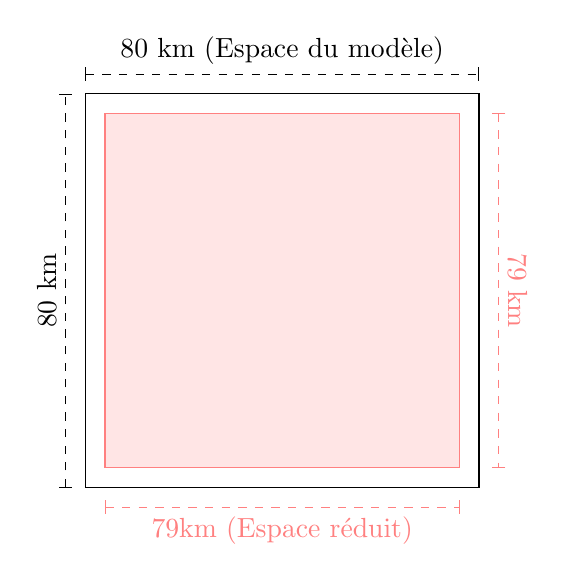
\begin{tikzpicture}[scale=.5]
\draw[] (0,0) -- (0,10) -- (10,10) -- (10,0) -- cycle;
\draw[|-|, very thin, dashed] (0, 10.5) -- node[above] {80 km (Espace du modèle)} (10, 10.5);
\draw[|-|, very thin, dashed] (-0.5, 0) -- node[above, rotate=90] {80 km} (-0.5, 10);

\draw[color=red!50, fill = red!10] (0.5, 0.5) -- (0.5, 9.5) -- (9.5, 9.5) -- (9.5, 0.5) -- cycle;
\draw[|-|, very thin, dashed, red!50] (10.50, 9.50) -- node[above, red!50, rotate=-90] {79 km} (10.5, 0.5);
\draw[|-|, very thin, dashed, red!50] (0.5, -0.5) -- node[below, red!50] {79km (Espace réduit)} (9.5, -0.5);
\end{tikzpicture}
\caption{L'espace support de SimFeodal, un monde théorique.\\
N.B : Dans le schéma, pour une question de lisibilité, les dimensions de l'espace réduit ne sont pas proportionnelles à celles de l'espace d'ensemble.}
\label{fig:espace-simfeodal}
\end{figure}

\paragraph[Endogène]{} Notons enfin que l'espace est strictement \textbf{endogène} au modèle. On entend par là que le monde n'est pas résultant du chargement d'un fichier géographique ou d'un paramétrage précis : seul un paramètre, qui régit la taille des côtés, joue sur la géométrie de l'espace.
Il nous semble important de le préciser, en particulier parce que c'est, à notre connaissance, assez inhabituel dans la simulation de données géographiques, mêmes théoriques : les agents sont placés de manière strictement aléatoire (via un aléa contrôlé tout de même) dans l'espace du modèle, et dès lors, aucune localisation ou surface ne sont identiques ou comparables d'une simulation à l'autre.


\subsubsection{Granularité temporelle}

SimFeodal modélise des processus qui se déroulent sur le temps long, et à ce titre, la gestion de la temporalité y est importante.
Le modèle inscrit son exécution dans une étendue de \textbf{400 ans}, \textbf{discrétisée} sous la forme de 20 pas de temps de \textbf{20 ans} chacun.

\paragraph[Durée]{} La période d'étude, thématique, s'étend entre 800 après J.-C. et 1100, qui correspondent à des repères temporels entre lesquels on estime que le plus gros de la transition étudiée s'est déroulée.
Pour modéliser ces évolutions, nous avons choisi de commencer à la même date, mais de prolonger l'exécution du modèle d'un siècle, portant donc l'intervalle modélisé à \textbf{400 ans}, \textbf{de 800 à 1200}\footnote{
	Dans les versions précédentes de SimFeodal, \textcite{cura_transition_2017} notamment, cette date était fixée à 1160. Nous avons choisi de prolonger de 40 ans parce que cela nous permet de comparer l'état final du modèle au début du XIII$^e$ siècle, et qu'on obtient ainsi un nombre de pas de temps plus \og rond\fg{} (20) qu'auparavant (18), ce qui permet par exemple de représenter l'évolution d'une simulation de manière plus régulière.
}. Prolonger cette date d'observation permet d'analyser le comportement du modèle après la période d'étude, et par exemple de voir si les processus à l'œuvre subissent bien un ralentissement, marquant par exemple la fin de la féodalité, plutôt qu'un accroissement constant.

\paragraph[Discret]{} Contrairement à la gestion de l'espace, nous avons choisi de modéliser le temps sous forme \textbf{discrète}.
On peut justifier ce choix avec deux raisons principales.
En premier lieu, la transition s'inscrit dans une forte incertitude temporelle. Les experts thématiques peuvent certes s'appuyer sur des dates précises, par exemple pour des années de réformes, mais les processus à l'œuvre s'inscrivent dans une durée floue, dont la résolution est difficilement réductible à moins d'un demi-siècle, et à peine meilleure pour des éléments matériels.
Avoir une vision continue du temps s'inscrirait ainsi dans une certaine sur-détermination du modèle en rapport aux connaissances thématiques sur lesquelles il s'appuie.
En second lieu, les processus sont modélisés à la résolution de \og foyers paysans\fg{}, c'est-à-dire à l'échelle de foyers plus que d'individus. Les migrations des foyers paysans correspondent empiriquement plutôt à des déplacements qui surviennent à l'échelle temporelle de la génération, c'est-à-dire que ces migrations se réalisent en fait quand les descendants d'un foyer s'établissent dans une nouvelle localisation.
La prise en compte d'un temps continu impliquerait donc la mise en place de bien plus de mécanismes probabilistiques, avec des aberrations potentielles plus importantes en terme de trajectoires des agents.

\paragraph[Pas de temps de 20 ans]{} Cette deuxième justification participe au choix de la granularité du modèle. \textbf{Les pas de temps ont une durée de 20 ans}, ce qui correspond à peu près à la durée d'une génération de l'époque.
Cela correspond aussi à la précision globale que l'on peut avoir sur l'apparition d'éléments matériels tels que les églises, paroisses et châteaux\footnote{
Certains de ces éléments sont connus avec une précision bien supérieure, par exemple quand des textes historiques mentionnent leur création. Ce n'est toutefois pas généralisé, et la granularité moyenne gravite donc plutôt autour de 20 à 40 ans.
}.
Dans l'ensemble, au vu des connaissances historiques, ces pas de temps doivent être interprétés comme des repères temporels plus que comme des dates précises. Que les premiers châteaux apparaissent en 980 ou en 1000 n'a pas d'importance dans le modèle, dans que cela se déroule avant la seconde moitié du XI$^e$ siècle par exemple.


La \cref{fig:frise-chrono} illustre les processus et événements qui surviennent pendant l'ensemble de cette période.

\begin{figure}[H]
	\centering
	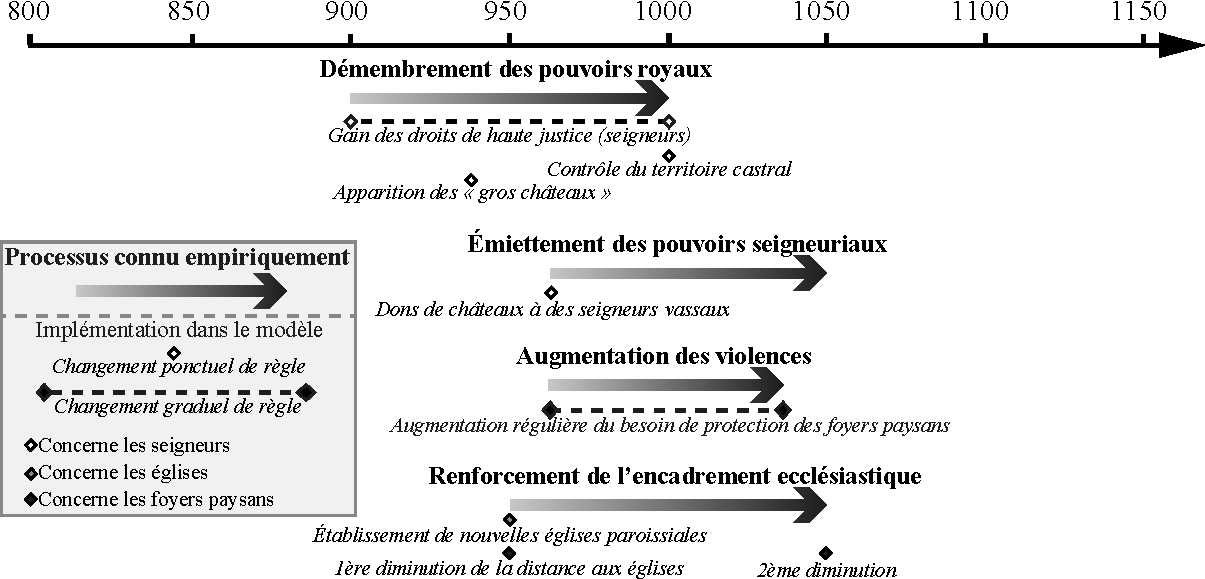
\includegraphics[width=\linewidth]{img/frise_chrono_tmd.pdf}
	\caption{Frise chronologique des processus historiques observés en Touraine implémentés dans SimFeodal. \hl{Figure issue de Peupler la Terre, à corriger/adapter.}}
	\label{fig:frise-chrono}
\end{figure}


\section[Fonctionnement général -- \textit{Process overview and schedulling}]{Fonctionnement général\protect\newline \large{\textit{Process overview and schedulling}} \sectionmark{Fonctionnement général}}

SimFeodal est un modèle qui s'inscrit plutôt dans une approche KIDS que KISS (\hl{voir chapitre 1}).
Il est donc constitué d'une large variété d'agents (\cref{tab:agents-simfeodal}), dotés pour certains de nombreux comportements.
Au total, ce sont près de quarante mécanismes particuliers (ici regroupés en une quinzaine de mécanismes généraux), appelés selon un ordonnancement constant, qui font interagir les agents à chaque pas de temps.
Dans cette partie, nous présentons une synthèse de ces mécanismes, sans entrer dans le détail, algorithmique ou mathématique, de chacun (voir la \cref{sec:meca-specifiques} pour des descriptions plus précises des mécanismes les plus complexes et importants).

\subsection{Ordonnancement général}

\begin{figure}[H]
	\centering
	% Couleurs
	\definecolor{bleuciel}{HTML}{a6cee3}
	\definecolor{mauve}{HTML}{1f78b4}
	\definecolor{beige}{HTML}{b2df8a}
	\definecolor{vert}{HTML}{33a02c}
	\definecolor{rose}{HTML}{fb9a99}
	\definecolor{rouge}{HTML}{e31a1c}
	% Styles des noeuds et lignes
	\tikzstyle{block} = [rectangle, draw, minimum width=4em, align=center, rounded corners, minimum height=2em, thick]
	\tikzstyle{start} = [draw, circle, minimum height=2em, align=center, thick]
	\tikzstyle{temp} = [very thick, dashed]
	\tikzstyle{line} = [draw, -{Latex[length=2.5mm,width=2.5mm]}]
	\tikzstyle{dline} = [draw, -{Latex[length=2.5mm,width=2.5mm,black!50]}, black!50, densely dotted]
	% 
	\tikzstyle{fps} = [fill=bleuciel]
	\tikzstyle{agregats} = [fill=mauve]    
	\tikzstyle{seigneurs} = [fill=vert]
	\tikzstyle{globals} = [fill=rouge!80]
	\tikzstyle{eglises} = [fill=rose!80]
	\tikzstyle{zps} = [fill=beige]
	\begin{tikzpicture}[node distance = .75cm and .75cm, auto, scale=0.7,every node/.style={transform shape}]
	% Place nodes
	\node [start, fill=rouge!80] (init) at (0,0) {Init.\\du\\monde};
	
	\node [start ,right= of init] (start) {Début\\du tour};
	\node [block, globals,right= of start] (maj-globals) {MaJ des \\variables\\globales};
	\node [block, fps, right= of maj-globals] (renouvellement-fp) {Renouvellement\\des FP};
	\node [block, eglises,right= of renouvellement-fp] (maj-paroisses) {MaJ des\\contours des\\paroisses};
	\node [block, agregats, right = of maj-paroisses] (maj-poles) {Détection\\des\\Pôles};
	
	\node [block, fps, below= of maj-poles] (maj-satisfaction) {MaJ satisfactions des FP};
	\node [block, fps, below=of maj-satisfaction] (migration-fp) {Migration des FP};
	\node [block, seigneurs, temp, below =of migration-fp] (maj-droits) {Gains de \\droits des seigneurs};
	\node [block, seigneurs, below=of maj-droits] (maj-zp) {Collecte des droits};
	
	\node [block, seigneurs, left=of maj-zp] (maj-dons) {Dons droits\\ et châteaux\\des Seigneurs};
	\node [block, globals, temp, left=of maj-dons] (promo-chateaux) {Promotion\\des châteaux};
	\node [block, seigneurs, temp, left=of promo-chateaux] (constructions-chateaux) {Construction\\ de châteaux};
	\node [block, seigneurs, left=of constructions-chateaux] (creation-seigneurs) {Création des\\nouveaux Seigneurs};		
	
	\node [block, agregats, above= of creation-seigneurs] (maj-agregats) {MaJ des Agrégats};
	\node [block, agregats, above=of maj-agregats] (maj-poles2) {MaJ des Pôles};
	\node [block, globals, above= of maj-poles2] (maj-outputs) {MaJ et enregistrement\\des \textit{outputs}};

	
	\path[line]%
	(maj-globals) -- (renouvellement-fp)
	(renouvellement-fp) -- (maj-paroisses)
	(maj-paroisses) -- (maj-poles)
	(maj-poles) -- (maj-satisfaction)
	(maj-satisfaction) -- (migration-fp)
	(migration-fp) -- (maj-droits)
	(maj-droits) -- (maj-zp)
	(maj-zp) -- (maj-dons)
	(maj-dons) -- (promo-chateaux)
	(promo-chateaux) -- (constructions-chateaux)
	(constructions-chateaux) -- (creation-seigneurs)
	(creation-seigneurs) -- (maj-agregats)
	(maj-agregats) -- (maj-poles2)
	(maj-poles2) -- (maj-outputs);

	
	\path[line] (init)-- (start);
	\path[line] (start) -- (maj-globals);
	\path[dline] (maj-outputs)-- (start);	
	\end{tikzpicture}
	\caption[a]{Ordonnancement des mécanismes de SimFeodal.\\
	{\footnotesize
	\colorbox{rouge!80}{\strut Mécanisme global} \colorbox{bleuciel}{\strut Foyers Paysans} \colorbox{rose!80}{\strut Églises} \colorbox{mauve}{\strut Agrégats et Pôles} \colorbox{vert}{\strut Seigneurs} \dbox{\strut Temporaire}
	}
	}
	\label{fig:ordonnancement}
\end{figure}
\setcounter{subsubsection}{-1}

Dans SimFeodal, les mécanismes sont toujours appelés dans le même ordre (voir \cref{fig:ordonnancement}) : l'ensemble de l'ordonnancement ne change pas tout au long des 20 pas de temps du modèle.
Certains mécanismes sont toutefois temporaires, c'est-à-dire rendus inactifs en fonction des pas de temps : la construction des châteaux, par exemple, n'est pas possible avant 940.
Jusqu'au pas de temps correspondant, le mécanisme est donc désactivé par un paramètre réglable.
Notons que si les mécanismes suivent un ordre déterminé, ce n'est pas le cas des agents qui sont appelés dans chacun : pour un mécanisme donné, l'ordre d'appel des agents est aléatoire et varie à chaque appel de ce mécanisme.


\subsubsection{Initialisation}

L'initialisation du monde consiste à créer le monde théorique dans lequel les agents vont interagir et à générer ces derniers.
Pendant cette étape, des foyers paysans sont générés dans l'espace du modèle :  une très large proportion est instanciée de manière dispersée et aléatoire, et quelques dizaines d'agents sont localisés de manière agrégés afin de constituer les premiers agrégats de population, de tailles variables (une vingtaine de villages peu peuplés et quelques agglomérations secondaires antiques plus importantes).
Lors de l'initialisation sont aussi créés les premiers seigneurs -- grands seigneurs sans portée spatiale et petits seigneurs localisés aléatoirement dans l'espace -- et les zones de prélèvement dans lesquelles ils prélèveront des droits divers.
L'initialisation est enfin l'occasion de créer et de disperser dans l'espace des églises (150), parmi lesquelles quelques-unes (50) se verront doter de droits paroissiaux et constitueront donc un premier maillage paroissial.

L'initialisation du monde est appelée une seule fois, avant que les pas de temps ne débutent. Elle repose fortement sur l'aléatoire, et génère donc une configuration spatiale différente à chaque nouvelle exécution du modèle (voir le paragraphe sur l'endogénéité de la \cref{subsec:reso-spatiale}).
Le détail de l'initialisation est décrit dans une partie ultérieure (\cref{sec:initialisation}), entièrement consacrée à ce mécanisme.

\subsubsection{Variables globales}

Plusieurs mécanismes de SimFeodal dépendent du temps : la possibilité, évoquée plus haut, pour les seigneurs de construire un château, mais aussi, entre autre, l'évolution des distances que les foyers paysans sont prêts à parcourir pour se rendre à l'église, ce qui permet de formaliser l'impact des réformes grégoriennes.
La mise en place de mécanismes tributaires de dates nous permet ainsi de représenter des événements exogènes au modèle qui peuvent ainsi servir de déclencheurs ou de catalyseurs à des processus de longue durée.
L'incrémentation de la date et la mise à jour des différentes variables temporelles, par exemple en sélectionnant les valeurs de ces différentes variables dans des tableaux de correspondance temporels, constituent donc la première étape de chaque nouveau pas de temps.

\subsubsection{Renouvellement des foyers paysans}

ABC

\subsubsection{Actualisation des paroisses}

\subsubsection{Détection des Pôles}

\subsubsection{Satisfaction des Foyers Paysans}

\subsubsection{Migration des Foyers Paysans}

\subsubsection{Gains de droits}

\subsubsection{Collecte des droits}

\subsubsection{Dons entre seigneurs}

\subsubsection{Promotion des châteaux}

\subsubsection{Construction de châteaux}

\subsubsection{Création de nouveaux seigneurs}

\subsubsection{Détection des agrégats}

\subsubsection{Actualisation des pôles}

\subsubsection{Enregistrement des \textit{outputs}}


\section[Design -- \textit{Design concepts}]{Design \protect\newline \large{\textit{Design concepts}} \sectionmark{Design}}

\subsection*{Basic principles}
\subsection*{Emergence}
\subsection*{Adaptation}
\subsection*{Objectives}
\subsection*{Learning}
\subsection*{Prediction}
\subsection*{Sensing}
\subsection*{Interaction}
\subsection*{Stochasticity}
\subsection*{Collectives}
\subsection*{Observation}


\section[Situation initiale -- \textit{Details - Initialisation}]{Situation initiale\protect\newline \large{\textit{Details - Initialisation}} \sectionmark{Situation initiale} \label{sec:initialisation}}

\subsection{Une situation initiale théorique et endogène}
a
\subsection{Paramètres d'initialisation}
a
\section[Données en entrée -- \textit{Input data}]{Données en entrée\protect\newline \large{\textit{Input data}} \sectionmark{Données en entrée}}
a

\section[Mécanismes spécifiques -- \textit{Submodels}]{Mécanismes spécifiques\protect\newline \large{\textit{Submodels}} \sectionmark{Mécanismes spécifiques} \label{sec:meca-specifiques}}

\subsection{Introduction} : Pas tout résumé ici

\subsection{Mécanismes globals}
	\subsubsection{Identification des agrégats}
	\subsubsection{Identification des pôles}
	\subsubsection{Identification des églises paroissiales}
	\subsubsection{Création et promotion d'églises paroissiales}

\subsection{Foyers paysans}
	\subsubsection{Renouvellement des foyers paysans}
	\subsubsection{Satisfaction et modèles gravitaires}
	\subsubsection{Déplacement des foyers paysans}

\subsection{Seigneurs}
	\subsubsection{Construction de châteaux}
	\subsubsection{Dons de châteaux}
	\subsubsection{Création et dons de droits}
	\subsubsection{Prélèvement des loyers}
	\subsubsection{Prélèvement des droits}

\printbibliography[title={Références}]
